\documentclass[../template]{subfiles}

\begin{document}
\section{Minimum Spanning Tree}

\begin{center}
    \begin{tikzpicture}[rotate=90]
        \Vertices[unit=2.3]{circle}{A,B,C,D,E}
        %\Edges(A,B,C,D,E)
        \Edge[color=red, label=$10$](A)(C)
        \Edge[label=$8$](A)(D)
        \Edge[color=red, label=$7$](D)(E)
        \Edge[color=red, label=$4$](A)(E)
        \Edge[color=red, label=$3$](B)(A)
        \Edge[label=$9$](B)(D)
        \Edge[label=$5$](B)(E)
        ;
    \end{tikzpicture}
\end{center}
\subsection{Algoritmo}
\lstinputlisting{algorithms/mst.py}
\subsection{Analisi complessità}
pass

\end{document}
